\myChapter{État de l'art sur la génération d'applications web pilotées par des modèles}{}
\label{chap:chap2-revu}
\myMiniToc{mysection}{Sommaire}

\mySection{Introduction}{}

La génération d'applications web à partir de modèles de processus se situe au
croisement du BPM, de BPMN et du développement web. BPMN permet de représenter
le déroulement du travail, mais il ne suffit pas à décrire les interfaces, les
données, les règles d'accès et l'architecture d'une application complète
\cite{omg2013bpmn}. 

Ce chapitre analyse donc les travaux qui rapprochent les
modèles de processus des artefacts logiciels, afin d'en dégager les apports, les
limites et le positionnement de notre recherche.

\mySection{Démarche d'analyse des travaux existants}{}

La revue n'a pas cherché à rassembler tous les travaux sur BPMN, mais à analyser ceux qui répondent à une question centrale : comment un modèle de processus peut-il être transformé en application web ou en artefacts logiciels utilisables ? Le corpus retenu privilégie donc les travaux portant sur les moteurs de workflow, les transformations BPMN vers d'autres modèles, la génération de code, les applications web générées, les plateformes orientées processus et les approches low-code. La démarche s'inspire des recommandations de Kitchenham et Charters ainsi que de l'esprit de PRISMA, sans constituer une revue systématique exhaustive \cite{kitchenham2007,prisma2020}.

L'analyse des travaux s'est faite en trois étapes : comprendre l'objectif de chaque approche, identifier les artefacts réellement produits et examiner les limites récurrentes. Ces limites concernent notamment l'insuffisance d'informations dans les modèles BPMN, la couverture partielle des applications, la dépendance à certaines plateformes, les difficultés de régénération et la cohabitation entre code généré et code manuel.
\begin{table}[H]
\centering
\caption{Grille concrète de lecture des travaux étudiés}
\label{tab:chap2-grille-analyse}
\begin{tabularx}{\textwidth}{p{3.2cm}X}
\toprule
\textbf{Point observé} & \textbf{Question posée pendant la lecture} \\
\midrule
Point de départ & Le travail part-il d'un modèle BPMN seul, d'un processus enrichi, d'un modèle de données ou d'un autre artefact ? \\
Résultat obtenu & Produit-il une interface, une API, une application exécutable, un prototype ou seulement une méthode de transformation ? \\
Place de la plateforme & Le résultat dépend-il fortement d'un moteur, d'un framework ou d'un environnement low-code ? \\
Preuve apportée & Les auteurs valident-ils leur proposition par un cas d'étude, une expérimentation, une comparaison ou une revue ? \\
Limite retenue & Que reste-t-il à faire pour obtenir une application complète, maintenable et adaptable ? \\
\bottomrule
\end{tabularx}
\end{table}

La revue qui suit présente donc les travaux par familles, puis met en évidence les limites
qui se dégagent de leur comparaison.

\mySection{Revue de la littérature}{}

\subsection{Systèmes d'information orientés processus et plateformes d'exécution}

Les systèmes d'information orientés processus placent le déroulement du travail
au centre de l'organisation du logiciel. Ils s'inscrivent dans le domaine plus
large de la gestion des processus métier, qui couvre la découverte, la
modélisation, l'exécution, le suivi et l'amélioration des processus
\cite{aalst2013,dumas2018fundamentals}. Dans cette perspective, le modèle ne sert plus
uniquement à documenter une organisation : il peut devenir une définition
exécutable utilisée par un moteur de processus.

\subsubsection{Moteurs BPMS et plateformes d'exécution}

Les systèmes de gestion des processus métier, ou \textit{Business Process
Management Systems} (BPMS), tels que Camunda, Flowable, jBPM ou Activiti
interprètent des définitions de processus, créent des instances, distribuent des tâches et
conservent un historique d'exécution \cite{camunda2026modeler,flowable2026bpmn,jbpm2026docs,activiti2026docs}. Leur
principal apport réside dans la séparation entre la logique d'orchestration et
les services appelés au cours du processus. Cette séparation rend le
déroulement visible et facilite son suivi. Elle impose néanmoins aux
applications clientes de manipuler les notions propres au moteur, notamment
les instances, les variables et les tâches. La plateforme exécute ainsi le
processus sans nécessairement produire l'ensemble de l'application qui
l'entoure.

\begin{figure}[H]
\centering
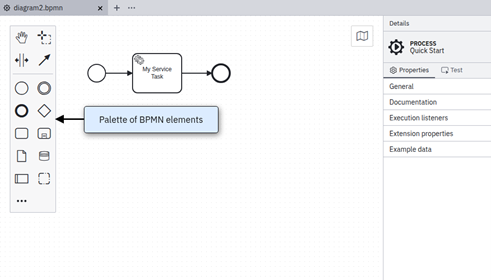
\includegraphics[width=0.75\textwidth]{Chap2/images/Image1.png}
\caption{Modélisation d'un processus BPMN exécutable dans Camunda Modeler, d'après la documentation Camunda \cite{camunda2026modeler}.}
\label{fig:chap2-camunda-modeler}
\end{figure}

La figure \ref{fig:chap2-camunda-modeler} montre le point d'entrée d'un moteur
comme Camunda : un processus BPMN enrichi de propriétés exécutables. Une fois
déployé, le moteur crée les instances, affecte les tâches et suit l'exécution,
mais il ne génère pas à lui seul toute l'application web qui l'exploite.

\subsubsection{Architecture web pilotée par BPMN}

Schäffer et al. proposent une architecture de référence et une méthode de
développement agile pour une plateforme web pilotée par BPMN
\cite{schaffer2021}. Leur travail montre comment associer une application web,
un moteur de processus et des services afin de conserver le processus comme
fil conducteur de l'implémentation. L'approche apporte une organisation
cohérente aux systèmes dont le comportement dépend fortement d'un workflow.
Elle reste toutefois centrée sur l'exécution et l'intégration du processus :
les autres dimensions de l'application doivent toujours être conçues et
développées autour de cette architecture.

\begin{figure}[H]
\centering
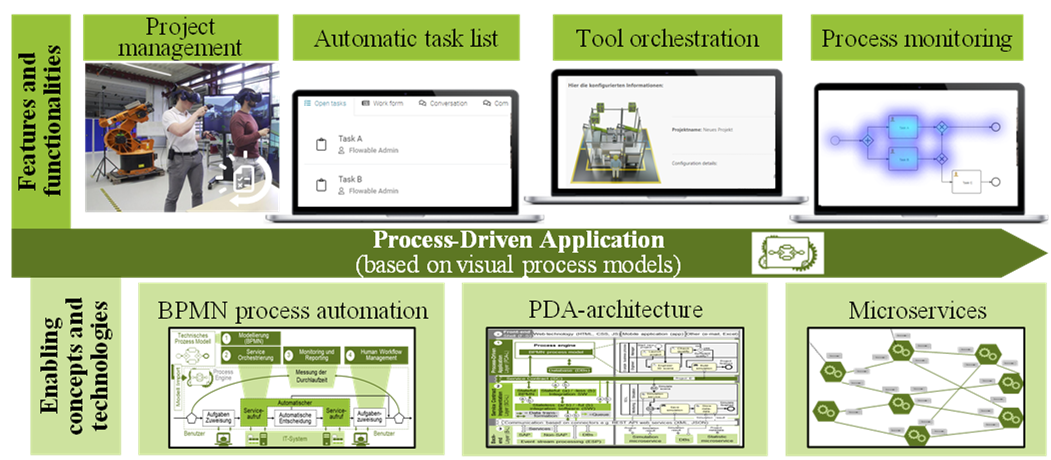
\includegraphics[width=0.75\textwidth]{Chap2/images/schaffer2021-process-driven-application.png}
\caption{Fonctionnalités et technologies d'une application web pilotée par processus \cite{schaffer2021}.}
\label{fig:chap2-schaffer-process-driven}
\end{figure}

La figure \ref{fig:chap2-schaffer-process-driven} montre qu'une application
pilotée par processus combine moteur BPMN, tâches, orchestration, supervision
et services. Le moteur de workflow y apparaît central, mais il doit être
entouré de composants applicatifs et d'intégration.

\subsubsection{WebWorkFlow}

WebWorkFlow adopte une direction différente. Hemel et al. considèrent qu'un
langage de workflow isolé n'est pas suffisant pour générer une application web
complète. Ils étendent donc WebDSL avec des abstractions de workflow, puis
traduisent ces abstractions vers les constructions du langage sous-jacent
\cite{hemel2008}. Cette intégration permet de générer des applications
personnalisées tout en couvrant les principaux patrons de contrôle de workflow.

\begin{figure}[H]
\centering
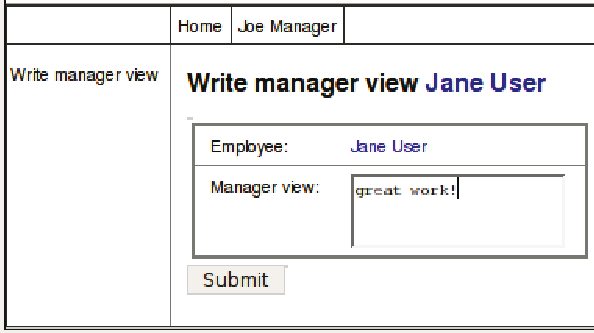
\includegraphics[width=0.75\textwidth]{Chap2/images/hemel2008-webworkflow-interface.png}
\caption{Interface générée dans WebWorkFlow pour une tâche de workflow, extraite de \cite{hemel2008}.}
\label{fig:chap2-webworkflow-interface}
\end{figure}

La figure \ref{fig:chap2-webworkflow-interface} illustre le résultat attendu :
une tâche de workflow devient une interface exploitable. L'apport est concret,
mais la portée de la génération reste liée au langage et aux abstractions de
WebDSL.

\subsubsection{Plateforme AKIP}

La plateforme ouverte AKIP, nom donné par ses auteurs, cherche à produire des
applications web orientées processus à partir de BPMN exécutable et de
spécifications complémentaires \cite{neto2022}. Son architecture associe un
générateur, un frontend, un backend, un moteur de processus, des connecteurs et
plusieurs fonctions transversales. Les auteurs répondent notamment aux
limites observées dans des plateformes existantes : dépendance envers un
fournisseur, interfaces peu flexibles, difficultés d'intégration et
technologies devenues anciennes.

\begin{figure}[H]
\centering
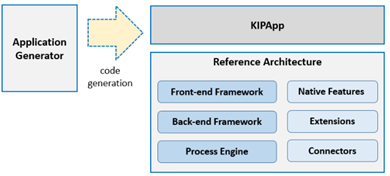
\includegraphics[width=0.75\textwidth]{Chap2/images/Image6.png}
\caption{Architecture et principe de génération d'une application dans AKIP, adaptés de \cite{neto2022}.}
\label{fig:chap2-akip}
\end{figure}

La figure \ref{fig:chap2-akip} montre une génération organisée autour d'une
architecture de référence. AKIP produit une base applicative moderne, mais son
évaluation reste limitée à une organisation et certaines constructions BPMN ne
sont pas encore couvertes.

Ces travaux montrent que l'exécution d'un processus est aujourd'hui bien
maîtrisée. Ils montrent également que le moteur ne résout qu'une partie du
problème applicatif. Plus une proposition vise une application complète, plus
elle doit associer au workflow des informations sur le domaine, les interfaces
et l'intégration technique.

\subsection{Dérivation d'artefacts applicatifs à partir de BPMN}

Une deuxième famille de recherches utilise BPMN comme point de départ pour
dériver des artefacts web précis. Ces travaux ne cherchent pas toujours à
générer l'ensemble d'un système. Ils étudient plutôt la manière dont les
éléments du processus peuvent fournir des informations utiles à la conception
d'interfaces, d'API ou de prototypes.

\subsubsection{Transformation vers des modèles d'interaction}

Sajji et al. proposent une transformation de BPMN vers l'\textit{Interaction
Flow Modeling Language} (IFML) dans le cadre de la \textit{Model Driven
Architecture} (MDA) \cite{sajji2022}. BPMN représente le niveau indépendant du
calcul, tandis qu'IFML décrit les vues, les événements utilisateur et les flux
d'interaction au niveau indépendant de la plateforme. Le travail établit des
règles de correspondance entre les éléments du processus et ceux de
l'interface. Il confirme que la structure du workflow peut guider la
construction de la navigation, mais que BPMN doit être complété pour exprimer
les détails de l'interaction.

%Dans un travail ultérieur, les mêmes auteurs prolongent la transformation
%jusqu'au niveau propre à une plateforme et génèrent des interfaces au moyen de
%WebRatio \cite{sajji2023}. L'étude de cas consacrée à une application de
%service après-vente illustre le passage progressif du processus à une interface
%exécutable. Cette continuité entre les niveaux de modèles constitue l'un des
%principaux résultats de l'approche. Sa portée demeure néanmoins concentrée sur
%les interfaces et les opérations de gestion de données ; elle ne traite pas
%entièrement le backend, la sécurité ou l'évolution de l'application générée.

Ces mêmes auteurs poursuivent cette logique en étudiant la transformation d'IFML
vers Symfony \cite{sajji2025}. L'intérêt de ce prolongement est de montrer que
le modèle d'interaction peut servir de point de départ à une génération
orientée framework web concret. La transformation s'appuie sur des règles ATL,
c'est-à-dire un langage utilisé pour définir des transformations entre modèles,
pour passer d'un modèle IFML indépendant de la plateforme vers un modèle
Symfony plus proche de l'implémentation.

\begin{figure}[H]
\centering
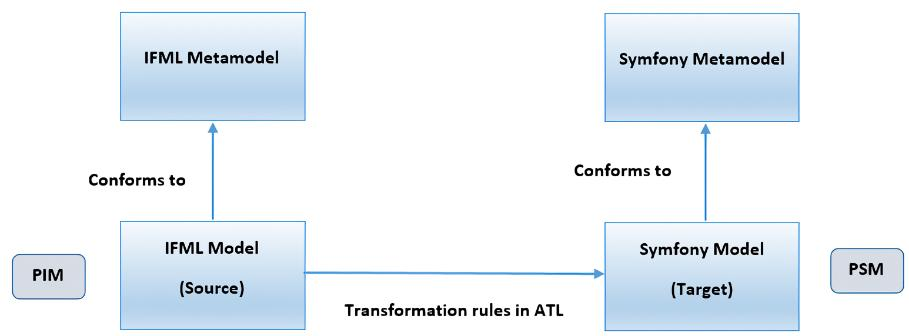
\includegraphics[width=0.75\textwidth]{Chap2/images/sajji2025-ifml-symfony.jpg}
\caption{Transformation d'un modèle IFML vers un modèle Symfony, adaptée de \cite{sajji2025}.}
\label{fig:chap2-ifml-symfony}
\end{figure}

La figure \ref{fig:chap2-ifml-symfony} illustre la logique MDA : IFML sert de
modèle indépendant, puis Symfony rapproche la représentation de l'implémentation.
Cette continuité réduit l'écart avec le code, mais renforce aussi la dépendance
aux conventions du framework cible.

Laaz et al. enrichissent les modèles BPMN avec des ontologies de domaine avant
de produire des modèles IFML \cite{laaz2020}. Les ontologies permettent de
préciser les concepts métier que le processus manipule sans les surcharger
directement dans le diagramme. Cette proposition répond à une faiblesse
récurrente de BPMN : les activités et les flux sont explicites, mais la
sémantique des données demeure souvent implicite. La qualité du résultat
dépend toutefois de la disponibilité et de la qualité de l'ontologie, dont la
construction représente elle-même un effort important.

\subsubsection{Génération de prototypes et d'API}

Díaz et al. associent les processus BPMN à des modèles structurels afin de
générer des prototypes d'interfaces graphiques \cite{diaz2018}. Leur travail
montre l'intérêt d'un prototype obtenu tôt dans le cycle de développement : il
permet de confronter le processus modélisé aux interactions attendues par les
utilisateurs. Le terme de prototype marque cependant la limite assumée de la
proposition. L'interface obtenue facilite la validation, mais elle ne constitue
pas encore une application complète prête à être exploitée.

Pietruck et Steffens s'intéressent à la génération d'API conformes au style
architectural \textit{Representational State Transfer} (REST) pour les moteurs
de workflow, à partir de modèles de processus et de données
\cite{pietruck2020}. Les API produites exposent des opérations plus proches du
domaine métier que les interfaces génériques d'un moteur. Cette abstraction
réduit le couplage entre les applications clientes et les concepts techniques
de son environnement d'exécution. Elle couvre cependant la couche d'accès au
processus et aux données, sans générer les interfaces utilisateur ni
l'ensemble des fonctions transversales.

\subsubsection{Vers une génération intégrée des artefacts applicatifs}

Hoyos et Restrepo-Calle proposent de générer automatiquement un prototype
d'application web orientée processus à partir d'une spécification rédigée dans
un langage naturel restreint \cite{hoyos2017}. Leur chaîne analyse la
spécification, extrait les informations utiles, puis produit des classes du
domaine, des formulaires, des vues et des contrôleurs.

\begin{figure}[H]
\centering
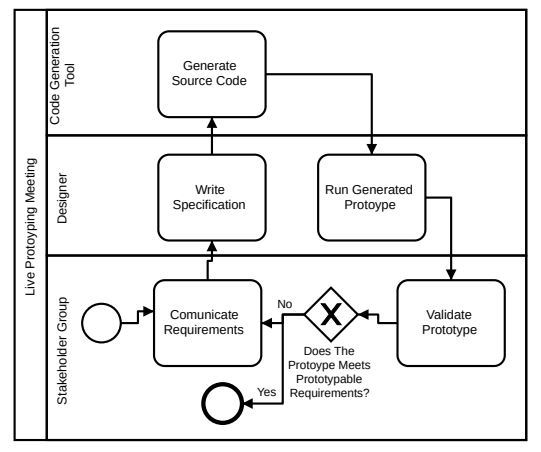
\includegraphics[width=0.70\textwidth]{Chap2/images/Image8.JPG}
\caption{Cycle de prototypage rapide d'applications web proposé par \cite{hoyos2017}.}
\label{fig:chap2-generation-hoyos}
\end{figure}

%La figure \ref{fig:chap2-generation-hoyos} présente le cycle suivi par les
%acteurs : expression des besoins, écriture de la spécification, génération du
%code, exécution puis validation du prototype. Elle montre surtout le caractère
%itératif de l'approche proposée.

\begin{figure}[H]
\centering
\begin{minipage}{0.48\textwidth}
\centering
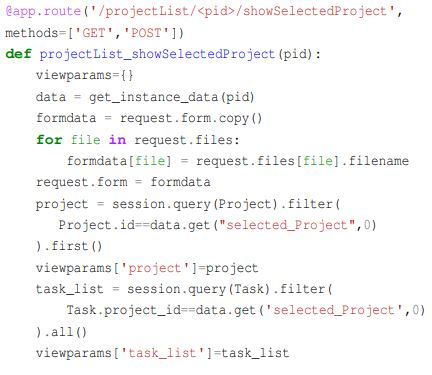
\includegraphics[width=\textwidth]{Chap2/images/image9.JPG}
\end{minipage}
\hfill
\begin{minipage}{0.48\textwidth}
\centering
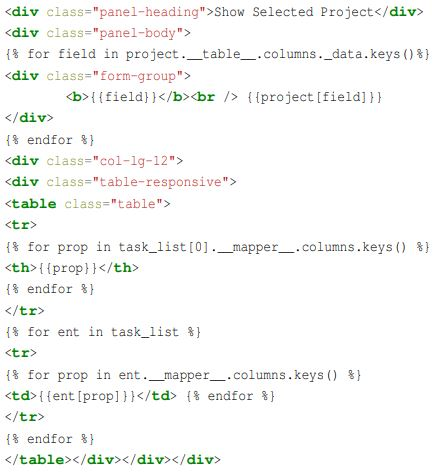
\includegraphics[width=\textwidth]{Chap2/images/image10.JPG}
\end{minipage}
\caption{Extraits de code généré pour le contrôleur et la vue dans l'approche de \cite{hoyos2017}.}
\label{fig:chap2-hoyos-code-genere}
\end{figure}

La figure \ref{fig:chap2-hoyos-code-genere} complète le cycle précédent en
montrant deux artefacts produits : une route côté contrôleur et un gabarit de
vue. Elle confirme que l'approche génère un prototype exploitable, même si la
qualité finale dépend encore des règles de génération.

Uyanik et Sayar développent un environnement web qui réunit conception
interactive du processus, gestion des flux et génération automatique de code
\cite{uyanik2023}. Dans leur contexte d'évaluation, les auteurs rapportent une
amélioration de 98,68\,\% du processus de développement, de 95,84\,\% pour les
conditions de test et de 36,01\,\% concernant la taille du code. Ces résultats
soulignent le potentiel d'une chaîne intégrée pour des applications
principalement organisées autour de formulaires et de processus. Ils restent
toutefois liés au protocole et au domaine évalués ; ils ne permettent pas
d'établir que les mêmes gains seraient obtenus pour des architectures plus
variées.

Pris ensemble, ces travaux confirment que BPMN contient des informations
exploitables pour produire plusieurs parties d'une application web. Ils
montrent aussi qu'une transformation ciblée conserve généralement une
couverture ciblée : l'interface, l'API ou le prototype progresse, tandis que
d'autres préoccupations restent hors du périmètre.

\subsection{Ingénierie dirigée par les modèles et génération de systèmes orientés processus}

L'ingénierie dirigée par les modèles considère les modèles comme des artefacts
productifs pouvant être validés, transformés et reliés au code. Cette
orientation est particulièrement adaptée aux systèmes orientés processus, car
elle permet d'associer plusieurs descriptions spécialisées au lieu d'exiger
qu'un seul modèle représente toute l'application.

\subsubsection{Composition de langages et génération progressive}

Drave et al. proposent une démarche générative pour les systèmes d'information
orientés processus \cite{drave2022}. Leur approche combine un langage textuel
pour BPMN avec des langages spécifiques décrivant notamment les structures de
données et les rôles. Les modèles sont contrôlés, transformés en
représentations intermédiaires, puis utilisés pour générer un système
extensible. Cette composition de langages vise à couvrir à la fois les
activités manuelles et automatisées, là où de nombreuses propositions se
concentrent sur une seule de ces dimensions.

\begin{figure}[H]
\centering
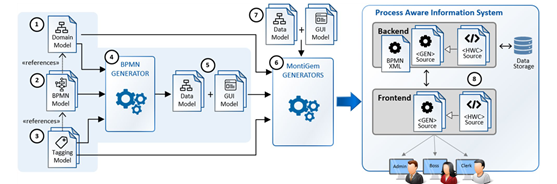
\includegraphics[width=0.75\textwidth]{Chap2/images/Image5.png}
\caption{Génération en deux étapes d'un système d'information orienté processus, adaptée de \cite{drave2022}.}
\label{fig:chap2-generation-drave}
\end{figure}

La figure \ref{fig:chap2-generation-drave} montre une génération en deux étapes
qui facilite le contrôle des transformations et la réutilisation des
informations. Sa limite tient à la couverture incomplète de BPMN et au coût de
maintenance des langages spécifiques mobilisés.

\subsubsection{Gabarits et compléments aux modèles BPMN}

La génération fondée sur des templates, c'est-à-dire des gabarits de fichiers
complétés automatiquement, reste l'une des techniques les plus utilisées pour
passer d'un modèle vers du code. L'étude de cartographie menée par Syriani et
al. montre que cette technique est répandue et qu'elle facilite l'adaptation
aux technologies cibles \cite{syriani2018}. Dans le cadre d'une génération
d'applications web métier, les gabarits ne sont toutefois utiles que s'ils
traduisent correctement les informations du processus en artefacts concrets :
routes, contrôleurs, formulaires, services, règles métier et accès aux données.
Leur maintenance devient alors un enjeu, car ils doivent évoluer avec les
cadres logiciels, les conventions de développement et la structure des modèles
d'entrée.

Plusieurs travaux montrent que le modèle de processus doit souvent être
complété pour produire une application exploitable. Fedeli et al. introduisent
des concepts propres aux environnements enrichis par l'Internet des objets
\cite{fedeli2024}, tandis que Salado-Cid et al. insistent sur la représentation
explicite des données, des opérations et des dépendances dans les workflows
intensifs en données \cite{salado2024}. Ces contributions ne visent pas
directement les applications web métier classiques, mais elles soulignent une
limite importante de BPMN : le flux de contrôle ne suffit pas toujours à
décrire les données manipulées, les interactions utilisateur et les contraintes
métier nécessaires à la génération.

Les travaux analysés font apparaître une limite récurrente : BPMN décrit efficacement le flux de contrôle, les activités, les événements, les passerelles et la répartition des responsabilités, mais il ne porte pas, à lui seul, toutes les informations nécessaires à la génération d'une application web métier. Dès que l'on cherche à produire des formulaires, à organiser la persistance, à contrôler les droits d'accès, à définir la visibilité des données ou à relier les sorties d'une activité aux entrées d'une autre, le modèle de processus doit être complété. Selon les approches, ce complément prend la forme de modèles de données, de modèles d'interaction, de métadonnées, de règles propres au domaine, de mappings ou de spécifications supplémentaires. Cette observation montre qu'une approche de génération ne peut pas demander à BPMN de tout décrire ; elle doit plutôt conserver BPMN comme modèle du processus et lui associer une description complémentaire des informations applicatives.

\subsection{Maintenabilité du code généré et mise en perspective avec le low-code}

La plupart des travaux de génération accordent une attention importante au
premier passage du modèle vers le code. Or, une application continue d'évoluer
après sa génération initiale. Les développeurs ajoutent des règles propres au
domaine, corrigent des comportements et adaptent les interfaces. En parallèle,
les processus et les technologies cibles changent. La coexistence du code
généré et du code écrit manuellement devient alors une question centrale.

\subsubsection{Gestion conjointe du code généré et du code manuel}

Greifenberg et al. comparent plusieurs mécanismes d'intégration du code
manuscrit et du code généré, notamment la séparation des fichiers, l'héritage,
la délégation et les zones protégées \cite{greifenberg2015}. Leur analyse
montre qu'aucun mécanisme ne répond parfaitement à toutes les situations.
Certains protègent clairement les modifications manuelles, mais imposent une
architecture plus complexe. D'autres offrent davantage de souplesse, au prix
d'un risque de conflit lors de la régénération. Le choix doit donc être prévu
dès la conception du générateur.

Rahad et al. étudient la place du développeur dans la boucle de l'ingénierie
dirigée par les modèles \cite{rahad2021}. Ils montrent que l'automatisation ne
supprime pas l'intervention humaine : celle-ci se déplace vers la vérification
des modèles, l'extension du code et la résolution des écarts entre le résultat
généré et le besoin réel. SeamlessMDD poursuit une préoccupation similaire en
cherchant à intégrer plus naturellement le code généré aux pratiques
habituelles de développement \cite{dragas2024}. Ces contributions rappellent
que la qualité d'une chaîne générative se mesure aussi après la première
génération.

Les travaux consacrés à l'intégration du code généré et du code manuscrit montrent que plusieurs stratégies peuvent être utilisées : séparation des fichiers, héritage, délégation, zones protégées, points d'extension ou mécanismes d'override. Aucune de ces stratégies n'est universelle. Leur pertinence dépend du type d'artefacts générés, du niveau de personnalisation attendu et de la fréquence des régénérations. Cette difficulté confirme que la maintenabilité doit être prise en compte dès la conception d'une chaîne de génération.

\subsubsection{Mise en perspective avec les approches low-code}

Les plateformes low-code cherchent également à réduire l'effort de développement grâce à des modèles visuels, composants et connecteurs \cite{rokis2023,pankowska2024}. Elles partagent avec l'IDM une recherche d'abstraction et d'automatisation. Toutefois, elles restent souvent dépendantes des plateformes, de leurs métamodèles, de leurs règles de gouvernance et de leurs connecteurs. Dans le cadre de ce mémoire, l'enjeu est différent : il s'agit de conserver des sources explicites, des transformations identifiables et des artefacts dont l'origine peut être inspectée. Cette différence situe le travail dans une logique d'ingénierie dirigée par les modèles plutôt que dans une démarche low-code généraliste.

\mySection{Discussion et positionnement de la recherche}{}

La littérature étudiée confirme qu'il est possible d'utiliser un modèle de
processus pour exécuter un workflow, produire des interfaces, exposer des API
ou générer une base applicative. Elle ne fait toutefois pas apparaître une
réponse unique couvrant, avec le même niveau de maturité, toutes les dimensions
d'une application web. Les propositions se distinguent surtout par le
compromis qu'elles établissent entre couverture, automatisation, flexibilité et
dépendance technologique.

Le tableau \ref{tab:chap2-travaux-etudies} montre que les travaux étudiés
apportent des réponses utiles, mais rarement complètes. Certains exécutent le
processus, d'autres génèrent une interface, une API ou un prototype. Les
approches les plus larges produisent une base applicative, mais elles restent
liées à une architecture, à un langage ou à une plateforme particulière.

\begin{table}[H]
\centering
\caption{Récapitulatif des travaux étudiés}
\label{tab:chap2-travaux-etudies}
\renewcommand{\arraystretch}{1.15}
\begin{tabularx}{\textwidth}{p{2.4cm}p{3.8cm}p{3.2cm}X}
\toprule
\textbf{Travail} & \textbf{Portée et résultat produit} & \textbf{Évaluation présentée} & \textbf{Limite principale} \\
\midrule
WebWorkFlow \cite{hemel2008} & Intégration d'abstractions de workflow à WebDSL pour générer des applications web personnalisées & Couverture des principaux patrons de contrôle de workflow & Dépendance au langage WebDSL et à ses abstractions \\
Sajji et al. \cite{sajji2022,sajji2023,sajji2025} & Transformation de BPMN vers IFML, puis d'IFML vers des technologies web comme WebRatio ou Symfony & Cas d'étude d'une application de service après-vente et règles de transformation vers Symfony & Couverture principalement limitée aux interactions et dépendance aux conventions de la plateforme cible \\
Hoyos et Restrepo-Calle \cite{hoyos2017} & Génération de classes, formulaires, vues et contrôleurs depuis un langage naturel restreint & Étude de cas démontrant la génération rapide d'un prototype & Langage d'entrée contraint et résultat orienté prototypage \\
Pietruck et Steffens \cite{pietruck2020} & Génération d'API REST orientées métier pour des moteurs de workflow & Démonstration de la transformation de modèles de processus et de données & Interfaces utilisateur et fonctions transversales hors du périmètre \\
%Drave et al. \cite{drave2022} & Génération progressive d'un système extensible à partir de BPMN et de langages complémentaires & Couverture annoncée de 89,5\,\% du BPMN analytique et de 86,8\,\% du BPMN exécutable & Multiplication des langages et nécessité de régénérer après évolution \\
Delgado et al. \cite{delgado2022} & Gestion dirigée par les modèles des familles de processus BPMN & Représentation de variantes proches d'un même processus & Configuration et contrôle de cohérence plus complexes \\
AKIP \cite{neto2022} & Génération d'une application web fonctionnelle intégrant interface, serveur et moteur de processus & Étude industrielle portant sur trois processus & Personnalisations métier nécessaires et couverture BPMN partielle \\
Uyanik et Sayar \cite{uyanik2023} & Environnement intégré de conception de processus et de génération de code & Gains importants rapportés pour le développement, les tests et la taille du code & Résultats liés à un contexte expérimental spécifique \\
Travaux low-code \cite{bucaioni2022,diruscio2022,pankowska2024,krouwel2024,martinez2026} & Usage de modèles visuels ou d'entreprise pour accélérer la construction d'applications & Revues et études de transformation vers des plateformes low-code & Dépendance aux plateformes, gouvernance et intégration persistantes \\
\bottomrule
\end{tabularx}
\end{table}

La comparaison des travaux étudiés ne permet pas seulement d'identifier des contributions isolées ; elle met aussi en évidence des limites récurrentes qui traversent plusieurs propositions. Ces limites concernent notamment l'insuffisance des informations portées par BPMN, la couverture partielle des artefacts générés, la dépendance à certaines plateformes, ainsi que les difficultés de traçabilité et de régénération. Le tableau~\ref{tab:chap2-synthese-critique} synthétise ces limites et en dégage les implications pour le framework à concevoir dans ce mémoire.

\begin{table}[H]
\centering
\caption{Limites transversales des travaux étudiés et implications pour la recherche}
\label{tab:chap2-synthese-critique}
\renewcommand{\arraystretch}{1.15}
\begin{tabularx}{\textwidth}{p{3.7cm}p{4.4cm}X}
\toprule
\textbf{Limite observée dans la littérature}
& \textbf{Conséquence pour la génération applicative}
& \textbf{Implication pour l'approche à concevoir} \\
\midrule

BPMN ne contient pas suffisamment d'informations applicatives.
& Les formulaires, les données, les rôles, les mappings et les règles de visibilité ne peuvent pas être déduits de manière fiable du diagramme seul.
& Prévoir une spécification complémentaire qui enrichit BPMN sans lui faire porter toute la description technique de l'application. \\

Les travaux génèrent souvent des fragments : interface, API ou prototype.
& Certaines couches de l'application restent hors du périmètre de génération et doivent être développées séparément.
& Viser une génération couvrant plusieurs couches du socle applicatif : interface, logique applicative, runtime, données et sécurité. \\

Certaines approches dépendent fortement d'une plateforme, d'un langage ou d'un framework.
& Le résultat obtenu devient difficile à transposer ou à faire évoluer hors de l'environnement prévu initialement.
& Séparer autant que possible les décisions métier des détails technologiques, au moyen de représentations intermédiaires et de règles de projection explicites. \\

La traçabilité entre modèles et fichiers générés reste souvent limitée.
& Lorsqu'un fichier est modifié ou régénéré, il devient difficile de retrouver l'élément du modèle qui l'a produit.
& Conserver des liens explicites entre les modèles sources, les représentations intermédiaires et les artefacts produits. \\

La cohabitation entre code généré et code manuel est difficile.
& Les adaptations du développeur peuvent être perdues ou entrer en conflit avec une nouvelle génération.
& Organiser dès le départ la séparation entre éléments générés, extensions manuelles et mécanismes de personnalisation. \\

La régénération après modification du modèle ou personnalisation du code est peu stabilisée.
& L'application peut se désaligner du processus ou écraser silencieusement des fichiers déjà adaptés.
& Prévoir une régénération contrôlée, capable d'identifier les fichiers suivis, les modifications locales et les conflits éventuels. \\

Les évaluations sont souvent limitées à un cas d'étude ou à un contexte spécifique.
& La généralisation des résultats doit rester prudente et dépend du domaine, du modèle et de l'environnement technique.
& Évaluer l'approche sur un cas suffisamment représentatif, tout en reconnaissant clairement les limites de généralisation. \\

\bottomrule
\end{tabularx}
\end{table}

% BPMN apparaît ainsi comme un point d'entrée pertinent, mais insuffisant pour
% produire seul une application web complète. Les travaux doivent souvent lui
% associer des modèles d'interaction, des modèles de données, des métadonnées ou
% des langages propres au domaine. Cette nécessité confirme que la génération ne
% peut pas reposer uniquement sur le diagramme de processus.

% Ce constat précise aussi le positionnement de ProOWeb. Un BPMS classique,
% comme Camunda, Flowable ou jBPM, fournit d'abord un moteur et des services pour
% déployer, exécuter et superviser des processus. ProOWeb poursuit un autre but :
% utiliser le processus comme source d'une chaîne de génération couvrant le socle
% backend/frontend, les données, les règles d'accès et les ressources du runtime.
% Il ne remplace donc pas un moteur de processus généraliste. De même, il se
% distingue d'une plateforme low-code par le caractère explicite et inspectable
% de ses sources BPMN et \textit{spec-v1}, de ses contrats intermédiaires et de
% ses transformations. Cette transparence facilite la traçabilité, mais elle
% demande un effort de modélisation et ne supprime pas les adaptations propres au
% projet.

% La limite la plus importante concerne l'évolution du résultat généré. Une
% application web doit pouvoir être modifiée, maintenue et parfois régénérée après
% un changement du processus. Or cette dimension reste peu stabilisée dans les
% travaux étudiés. Notre recherche se positionne donc dans cet espace : relier le
% modèle de processus aux artefacts applicatifs tout en gardant un code
% compréhensible, modifiable et maintenable.

\mySection{Conclusion}{}

Les travaux étudiés montrent que les modèles de processus peuvent guider l'exécution d'un workflow et soutenir la production d'interfaces, d'API, de prototypes ou de bases applicatives. Ils confirment aussi que BPMN constitue un point d'entrée pertinent pour représenter le fonctionnement métier. Cependant, ils révèlent plusieurs limites persistantes : le modèle BPMN doit être complété par des informations applicatives, la couverture générée reste souvent partielle, certaines solutions demeurent liées à une plateforme ou à un langage, la traçabilité modèle--code reste fragile et l'évolution du code généré demeure délicate.

%Ce chapitre permet donc de dégager le besoin d'une approche capable d'associer un processus BPMN à une spécification complémentaire, de contrôler leur cohérence, de produire des représentations intermédiaires exploitables et de projeter ces informations vers un socle applicatif web métier. Le chapitre suivant présente la réponse proposée à ce besoin, en détaillant l'architecture du framework, le modèle d'entrée enrichi, les transformations et les mécanismes prévus pour préserver la traçabilité et accompagner la régénération.

Ces exigences structurent la conception du framework ProOWeb, présenté au chapitre suivant comme la solution proposée dans ce mémoire pour générer un socle applicatif web métier à partir de modèles BPMN enrichis.
